%\documentclass[smaller, dvipsnames, handout]{beamer}
\def\bmode{0} % Mode 0 for presentation, mode 1 for a handout with notes, mode 2 fo% r handout without notes
\if 0\bmode
\immediate\write18{pdflatex -jobname=\jobname-Presentation\space\jobname}
\documentclass[usenames,dvipsnames,smaller]{beamer}
\else \if 1\bmode
\immediate\write18{pdflatex -jobname=\jobname-Handout-Notes\space\jobname}
\documentclass[usenames,dvipsnames,smaller,handout]{beamer}
\usepackage{handoutWithNotes}
\pgfpagesuselayout{2 on 1 with notes}[letterpaper, landscape, border shrink=4mm]
\else \if 2\bmode
\immediate\write18{pdflatex -jobname=\jobname-Handout\space\jobname}
\documentclass[usenames,dvipsnames,smaller,handout]{beamer}
\fi
\fi
\fi


%\setbeamertemplate{section in head/foot}{}
%\setbeamertemplate{section in head/foot shaded}{\textcolor{white}{\insertsectionhead}}
%%%%%%%%%%%%%%%%%%%%%%%%%%%%%%%%%%%%%%%%%%%%%%%%%%%%%%%%%%%%%%%%%%%%%%%%%%%%%%%%%%%%%%%%%%%%%
\newcommand{\coursetitle}{CEE 616: Probabilistic Machine Learning}
\newcommand{\longlecturetitle}{M5 Unsupervised Learning:\\ L5c:  Clustering}
\newcommand{\shortlecturetitle}{L5c: Clustering}
\newcommand{\instructor}{Jimi Oke}
\newcommand{\lecturedate}{Tue, Dec 9, 2025}
%%%%%%%%%%%%%%%%%%%%%%%%%%%%%%%%%%%%%%%%%%%%%%%%%%%%%%%%%%%%%%%%%%%%%%%%%%%%%%%%%%%%%%%%%%%%%


 
% \usepackage[T1]{fontenc} 
% \usepackage{lmodern} 
%\usepackage{etex}
 %\newcommand{\num}{6{} }

% \usetheme[
%   outer/progressbar=foot,
%   outer/numbering=fraction,
%   block=fill,
%   inner/subsectionpage=progressbar
% ]{metropolis}
\usetheme{Madrid}
\useoutertheme[subsection=false]{miniframes} % Alternatively: miniframes, infolines, split
\useinnertheme{circles}
% %\useoutertheme{Frankfurt}
% \usecolortheme{beaver}
% %\useoutertheme{crane}
% %\useoutertheme{metropolis}
\usepackage[backend=biber,style=authoryear,maxcitenames=2,maxbibnames=99,safeinputenc,url=false, eprint=false]{biblatex}
%\addbibresource{bib/references.bib}
% \AtEveryCitekey{\iffootnote{{\tiny}\tiny}{\tiny}}

% %\usepackage{pgfpages}
% %\setbeameroption{hide notes} % Only slides
% %\setbeameroption{show only notes} % Only notes
% %\setbeameroption{hide notes} % Only notes
% %\setbeameroption{show notes on second screen=right} % Both

% % \usepackage[sfdefault]{Fira Sans}

% % \setsansfont[BoldFont={Fira Sans}]{Fira Sans Light}
% % \setmonofont{Fira Mono}

% %\usepackage{fira}
% %\setsansfont{Fira}
% %\setmonofont{Fira Mono}
% % To give a presentation with the Skim reader (http://skim-app.sourceforge.net) on OSX so
% % that you see the notes on your laptop and the slides on the projector, do the following:
% % 
% % 1. Generate just the presentation (hide notes) and save to slides.pdf
% % 2. Generate onlt the notes (show only nodes) and save to notes.pdf
% % 3. With Skim open both slides.pdf and notes.pdf
% % 4. Click on slides.pdf to bring it to front.
% % 5. In Skim, under "View -> Presentation Option -> Synhcronized Noted Document"
% %    select notes.pdf.
% % 6. Now as you move around in slides.pdf the notes.pdf file will follow you.
% % 7. Arrange windows so that notes.pdf is in full screen mode on your laptop
% %    and slides.pdf is in presentation mode on the projector.

% % Give a slight yellow tint to the notes page
% \setbeamertemplate{note page}{\pagecolor{yellow!5}\insertnote}\usepackage{palatino}

% %\usetheme{metropolis}
% %\usecolortheme{beaver}
 \usepackage{tipa}
% \usepackage{enumerate}
\definecolor{darkcandyapplered}{HTML}{A40000}
\definecolor{lightcandyapplered}{HTML}{e74c3c}

% %\setbeamercolor{title}{fg=darkcandyapplered}

% \definecolor{UBCblue}{rgb}{0.04706, 0.13725, 0.26667} % UBC Blue (primary)
% \definecolor{UBCgrey}{rgb}{0.3686, 0.5255, 0.6235} % UBC Grey (secondary)

% % \setbeamercolor{palette primary}{bg=darkcandyapplered,fg=white}
% % \setbeamercolor{palette secondary}{bg=darkcandyapplered,fg=white}
% % \setbeamercolor{palette tertiary}{bg=darkcandyapplered,fg=white}
% % \setbeamercolor{palette quaternary}{bg=darkcandyapplered,fg=white}
% % \setbeamercolor{structure}{fg=darkcandyapplered} % itemize, enumerate, etc
% % \setbeamercolor{section in toc}{fg=darkcandyapplered} % TOC sections
% % \setbeamercolor{frametitle}{fg=darkcandyapplered,bg=white} % TOC sections
% % \setbeamercolor{title in head/foot}{bg=white,fg=white} % TOC sections
% % \setbeamercolor{button}{fg=darkcandyapplered} % TOC sections

% % % Override palette coloring with secondary
% % \setbeamercolor{subsection in head/foot}{bg=lightcandyapplered,fg=white}

%\usecolortheme{crane}
% \makeatletter
% \setbeamertemplate{headline}{%
%   \begin{beamercolorbox}[colsep=1.5pt]{upper separation line head}
%   \end{beamercolorbox}
%   \begin{beamercolorbox}{section in head/foot}
%     \vskip1pt\insertsectionnavigationhorizontal{\paperwidth}{}{}\vskip1pt
%   \end{beamercolorbox}%
%   \ifbeamer@theme@subsection%
%     \begin{beamercolorbox}[colsep=1.5pt]{middle separation line head}
%     \end{beamercolorbox}
%     \begin{beamercolorbox}[ht=2.5ex,dp=1.125ex,%
%       leftskip=.3cm,rightskip=.3cm plus1fil]{subsection in head/foot}
%       \usebeamerfont{subsection in head/foot}\insertsubsectionhead
%     \end{beamercolorbox}%
%   \fi%
%   \begin{beamercolorbox}[colsep=1.5pt]{lower separation line head}
%   \end{beamercolorbox}
% }
% \makeatother

% Reduce size of frame box
\setbeamertemplate{frametitle}{%
    \nointerlineskip%
    \begin{beamercolorbox}[wd=\paperwidth,ht=2.0ex,dp=0.6ex]{frametitle}
        \hspace*{1ex}\insertframetitle%
    \end{beamercolorbox}%
}


%\setbeamercolor{frametitle}{bg=darkcandyapplered!80!black!90!white}
%\setbeamertemplate{frametitle}{\bf\insertframetitle}

%\setbeamercolor{footnote mark}{fg=darkcandyapplered}
%\setbeamercolor{footnote}{fg=darkcandyapplered!70}
%\Raggedbottom
%\setbeamerfont{page number in head/foot}{size=\tiny}
%\usepackage[tracking]{microtype}


% %\usepackage[sc,osf]{mathpazo}   % With old-style figures and real smallcaps.
% %\linespread{1.025}              % Palatino leads a little more leading

% % Euler for math and numbers
% %\usepackage[euler-digits,small]{eulervm}
% %\AtBeginDocument{\renewcommand{\hbar}{\hslash}}
\usepackage{graphicx}
\usepackage{multirow}
\usepackage{booktabs}
\usepackage{graphbox}
\usepackage{animate}
\usepackage{media9}
\usepackage{adjustbox}

% %\mode<presentation> { \setbeamercovered{transparent} }

\setbeamertemplate{navigation symbols}{}
\makeatletter
\def\beamerorig@set@color{%
  \pdfliteral{\current@color}%
  \aftergroup\reset@color
}
\def\beamerorig@reset@color{\pdfliteral{\current@color}}
\makeatother


% %=== GRAPHICS PATH ===========
\graphicspath{{./m5-images/}}
% % Marginpar width
% %Marginpar width
% %\setlength{\marginparsep}{.02in}


% %% Captions
% % \usepackage{caption}
% % \captionsetup{
% %   labelsep=quad,
% %   justification=raggedright,
% %   labelfont=sc
% % }

% \setbeamerfont{caption}{size=\footnotesize}
% \setbeamercolor{caption name}{fg=darkcandyapplered}

% %AMS-TeX packages

\usepackage{amssymb}
\usepackage{amsmath}
\usepackage{amsthm}
\usepackage{mathtools} 
\usepackage{bm}
\DeclareMathOperator*{\argmax}{arg\,max}
\DeclareMathOperator*{\argmin}{arg\,min}
% \usepackage{color}

% %https://tex.stackexchange.com/a/31370/2269
\usepackage{cancel}
\renewcommand{\CancelColor}{\color{red}} %change cancel color to red
\makeatletter
\let\my@cancelto\cancelto %copy over the original cancelto command
\newcommand<>{\cancelto}[2]{\alt#3{\my@cancelto{#1}{#2}}{\mathrlap{#2}\phantom{\my@cancelto{#1}{#2}}}}
% redefine the cancelto command, using \phantom to assure that the
% result doesn't wiggle up and down with and without the arrow
\makeatother


% % \usepackage{comment}
\usepackage{enumerate}
\usepackage{hyperref}
% \usepackage{minitoc,array}
% \definecolor{slblue}{rgb}{0,.3,.62}
\hypersetup{
    colorlinks,%
    citecolor=blue,%
    filecolor=blue,%
    linkcolor=blue,
    urlcolor=blue
}

% \usepackage{epstopdf}
% \epstopdfDeclareGraphicsRule{.gif}{png}{.png}{convert gif:#1 png:\OutputFile}
% \AppendGraphicsExtensions{.gif}

% %\usepackage{listings}

% %%% TIKZ
\usepackage{forest}
\usepackage{tikz}
\usepackage{tikz-3dplot}
\usepackage{pgfplots}
\usepackage{pgfplotstable}
% \usepackage{pgfgantt}
\usepackage{neuralnetwork}

\usetikzlibrary{fit,arrows,arrows.meta,shapes,positioning,shapes.geometric}
\usetikzlibrary{decorations.markings}
\usetikzlibrary{shadows,automata}
\usetikzlibrary{patterns}
\usetikzlibrary{trees,mindmap,backgrounds}
%\usetikzlibrary{circuits.ee.IEC}
\usetikzlibrary{decorations.text}
% % For Sagnac Picture
% \usetikzlibrary{%
%     decorations.pathreplacing,%
%     decorations.pathmorphing%
% }
% \tikzset{no shadows/.style={general shadow/.style=}}
% %
% %\usepackage{paralist}

\tikzset{
  font=\Large\sffamily\bfseries,
  red arrow/.style={
    midway,red,sloped,fill, minimum height=3cm, single arrow, single arrow head extend=.5cm, single arrow head indent=.25cm,xscale=0.3,yscale=0.15,
    allow upside down
  },
  black arrow/.style 2 args={-stealth, shorten >=#1, shorten <=#2},
  black arrow/.default={1mm}{1mm},
  tree box/.style={draw, rounded corners, inner sep=1em},
  node box/.style={white, draw=black, text=black, rectangle, rounded corners},
}

% %%% FORMAT PYTHON CODE
% %\usepackage{listings}
% % Default fixed font does not support bold face
% \DeclareFixedFont{\ttb}{T1}{txtt}{bx}{n}{8} % for bold
% \DeclareFixedFont{\ttm}{T1}{txtt}{m}{n}{8}  % for normal

% % Custom colors
% \definecolor{deepblue}{rgb}{0,0,0.5}
% \definecolor{deepred}{rgb}{0.6,0,0}
% \definecolor{deepgreen}{rgb}{0,0.5,0}

% %\usepackage{animate}

% % Python style for highlighting
% % \newcommand\pythonstyle{\lstset{
% % language=Python,
% % basicstyle=\footnotesize\ttm,
% % otherkeywords={self},             % Add keywords here
% % keywordstyle=\footnotesize\ttb\color{deepblue},
% % emph={MyClass,__init__},          % Custom highlighting
% % emphstyle=\footnotesize\ttb\color{deepred},    % Custom highlighting style
% % stringstyle=\color{deepgreen},
% % frame=tb,                         % Any extra options here
%     % showstringspaces=false            % 
% % }}

% % % Python environment
% % \lstnewenvironment{python}[1][]
% % {
% % \pythonstyle
% % \lstset{#1}
% % }
% % {}

% % % Python for external files
% % \newcommand\pythonexternal[2][]{{
% % \pythonstyle
% % \lstinputlisting[#1]{#2}}}

% % Python for inline
% % 
% % \newcommand\pythoninline[1]{{\pythonstyle\lstinline!#1!}}

% %\usepackage{algorithm2e}

\newcommand{\eps}{\epsilon}
\newcommand{\bX}{\mb X}
\newcommand{\by}{\mb y}
\newcommand{\bbe}{\bm\beta}
\newcommand{\beps}{\bm\epsilon}
\newcommand{\bY}{\mb Y}

\newcommand{\osn}{\oldstylenums}
\newcommand{\dg}{^{\circ}}
\newcommand{\lt}{\left}
\newcommand{\rt}{\right}
\newcommand{\pt}{\phantom}
\newcommand{\tf}{\therefore}
\newcommand{\?}{\stackrel{?}{=}}
\newcommand{\fr}{\frac}
\newcommand{\dfr}{\dfrac}
\newcommand{\ul}{\underline}
\newcommand{\tn}{\tabularnewline}
\newcommand{\nl}{\newline}
\newcommand\relph[1]{\mathrel{\phantom{#1}}}
\newcommand{\cm}{\checkmark}
\newcommand{\ol}{\overline}
\newcommand{\rd}{\color{red}}
\newcommand{\bl}{\color{blue}}
\newcommand{\pl}{\color{purple}}
\newcommand{\og}{\color{orange!90!black}}
\newcommand{\gr}{\color{green!40!black}}
\newcommand{\lbl}{\color{CornflowerBlue}}
\newcommand{\dca}{\color{darkcandyapplered}}
\newcommand{\nin}{\noindent}
\newcommand*\circled[1]{\tikz[baseline=(char.base)]{
            \node[shape=circle,draw,thick,inner sep=1pt] (char) {\small #1};}}

\newcommand{\bc}{\begin{compactenum}[\quad--]}
\newcommand{\ec}{\end{compactenum}}

\newcommand{\p}{\partial}
\newcommand{\pd}[2]{\frac{\partial{#1}}{\partial{#2}}}
\newcommand{\dpd}[2]{\dfrac{\partial{#1}}{\partial{#2}}}
\newcommand{\pdd}[2]{\frac{\partial^2{#1}}{\partial{#2}^2}}
\newcommand{\pde}[3]{\frac{\partial^2{#1}}{\partial{#2}\partial{#3}}}
\newcommand{\nmfr}[3]{\Phi\left(\frac{{#1} - {#2}}{#3}\right)}
\newcommand{\Err}{\text{Err}}
\newcommand{\err}{\text{err}}

\DeclarePairedDelimiter\ceil{\lceil}{\rceil}
\DeclarePairedDelimiter\floor{\lfloor}{\rfloor}

%%%% GREEK LETTER SHORTCUTS %%%%%
\newcommand{\la}{\lambda}
\renewcommand{\th}{\theta}
\newcommand{\al}{\alpha}
\newcommand{\G}{\Gamma}
\newcommand{\si}{\sigma}
\newcommand{\Si}{\Sigma}


\pgfmathdeclarefunction{poiss}{1}{%
  \pgfmathparse{(#1^x)*exp(-#1)/(x!)}%
  }

\pgfmathdeclarefunction{gauss}{2}{%
  \pgfmathparse{1/(#2*sqrt(2*pi))*exp(-((x-#1)^2)/(2*#2^2))}%
}

\pgfmathdeclarefunction{expo}{2}{%
  \pgfmathparse{#1*exp(-#1*#2)}%
}

\pgfmathdeclarefunction{expocdf}{2}{%
  \pgfmathparse{1 -exp(-#1*#2)}%
}

\newcommand{\mb}{\mathbb}
\newcommand{\mc}{\mathcal}
\newcommand{\tr}{^{\top}}
\newcommand{\empt}[2]{$#1^{( #2 )}$}
\newcommand{\pe}{\pause}
% \usepackage{pst-plot}

% \usepackage{pstricks-add}
% \usepackage{auto-pst-pdf}   

% \psset{unit = 3}

% \def\target(#1,#2){%
%  {\psset{fillstyle = solid}
%   \rput(#1,#2){%
%     \pscircle[fillcolor = white](0.7,0.7){0.7}
%     \pscircle[fillcolor = blue!60](0.7,0.7){0.5}
%     \pscircle[fillcolor = white](0.7,0.7){0.3}
%     \pscircle[fillcolor = red!80](0.7,0.7){0.1}}}}
% \def\dots[#1](#2,#3){%
%     \psRandom[
%       dotsize = 2pt,
%       randomPoints = 25
%     ](!#2 #1 0.04 sub sub #3 #1 0.04 sub sub)%
%      (!#2 #1 0.04 sub add #3 #1 0.04 sub add)%
%      {\pscircle[linestyle = none](#2,#3){#1}}}


%%%%%%%%%%%%%%%%%%%%%%%%%%%%%%%%%%%%%%%%%%%%%%%%%%%
%%%%%%%%%%%%%%%%%%%%%%%%%%%%%%%%%%%%%%%%%%%%%%%%%%%
\title[\shortlecturetitle]{ {\normalsize \coursetitle}
  \\ \longlecturetitle}
\date[\lecturedate]{\footnotesize \lecturedate}
\author{{\bf \instructor}}
\institute[UMass Amherst]{
%\titlegraphic{\hfill
  \begin{tikzpicture}[baseline=(current bounding box.center)]
    \node[anchor=base] at (-7,0) (its) {\includegraphics[scale=.3]{UMassEngineering_vert}} ;
  \end{tikzpicture}
  % \hfill\includegraphics[height=1.5cm]{logo}
}

%https://tex.stackexchange.com/questions/55806/mindmap-tikzpicture-in-beamer-reveal-step-by-step
  \tikzset{
    invisible/.style={opacity=0},
    visible on/.style={alt={#1{}{invisible}}},
    alt/.code args={<#1>#2#3}{%
      \alt<#1>{\pgfkeysalso{#2}}{\pgfkeysalso{#3}} % \pgfkeysalso doesn't change the path
    },
  }


% https://tex.stackexchange.com/questions/446468/labels-with-arrows-for-an-equation
% https://tex.stackexchange.com/a/402466/121799
\newcommand{\tikzmark}[3][]{
\ifmmode
\tikz[remember picture,baseline=(#2.base)] \node [inner sep=0pt,#1](#2) {$#3$};
\else
\tikz[remember picture,baseline=(#2.base)] \node [inner sep=0pt,#1](#2) {#3};
\fi
}

% \lstset{language=matlab,
%                 basicstyle=\scriptsize\ttfamily,
%                 keywordstyle=\color{blue}\ttfamily,
%                 stringstyle=\color{blue}\ttfamily,
%                 commentstyle=\color{gray}\ttfamily,
%                 morecomment=[l][\color{gray}]{\#}
%               }


%%% Local Variables:
%%% mode: latex
%%% TeX-master: t
%%% End:

%\setbeamercolor{local structure}{fg=white}

\begin{document}
\maketitle
\begin{frame}
  \frametitle{Outline}
  \tableofcontents
\end{frame}



\section{Introduction}

%%% SLIDE LAYOUT EXAMPLE
\begin{frame}{What is Clustering? } \pause
 \begin{itemize}
   % \setlength{\itemindent}{-1em}
 \item \alert{Exploratory} technique to discover useful relationships in data \pause
 \item Can also be used for classification \pause
   \item Clustering means grouping $n$ observations into homogeneous partitions \pause
   \item There is no dependent variable, $y$ (\emph{unsupervised learning}) \pause
   \item Observations $\mathbf{x}_j$ are grouped based on similarity \pause
    \end{itemize}
 
    \pause
    \begin{alertblock}{}
      \begin{itemize}
          % \item Clustering is based on \alert{similarity measures} (the main input into a clustering algorithm).
  \item Objective: \pause
  \begin{itemize}
   \item high similarity between items that belong to the same cluster \pause
   \item low similarity (high separation) between different clusters \pause
   \end{itemize}
 \end{itemize}
\end{alertblock}
 
\end{frame}




\begin{frame}
  \frametitle{Clustering Application: Marketing} \pause
  
  \begin{itemize}
  \item \alert{Customer segmentation} based on brand loyalty and price sensitivity scores.
  \end{itemize}
  \centering
  \includegraphics<3->[height=6cm]{customer}
\newline
\tiny{Source: \url{http://www.select-statistics.co.uk/}}
\end{frame}



\section{Similarity measures}

\begin{frame}[shrink=5]
\frametitle{Similarity Measures}
 \begin{columns}     %[T] for top vertical alignment
  \begin{column}{0.48\textwidth}
    \begin{itemize}
      %\item The choice of a similarity measure is important and can lead to different clusters.
      \item How similar are two observations?
      \begin{itemize}
        \item Geographical distance
        \item Vehicle color
        \item Vehicle type
        \item Vehicle brand
        \item Engine type
        \item Engine power
        \item ...
      \end{itemize}
%    \item MIT \emph{Tech Shuttle} bus:
%    \begin{itemize}
%    \item Geographical distance
%    \end{itemize}
    \end{itemize}
  \end{column}
 \begin{column}{0.48\textwidth}
  \begin{figure}
    \includegraphics[width=1.0\columnwidth]{parking}
    \caption{Vehicles as items for cluster analysis}
  \end{figure}
  \end{column}
 \end{columns}
\end{frame}


\begin{frame}
  \frametitle{Similarity measures: numerical/quantitative data} \pause
  Comparing two vectors, $\textbf{x}_i$ and $\textbf{x}_k$, with $p$ variables/features:\pause

  \begin{itemize}
  \item \textbf{Euclidean distance} \pause
    \begin{equation}
      d(\mathbf{x}_i, \mathbf{x}_k)= \pause \sqrt{\sum\limits_{j=1}^p(x_{ij}-x_{kj})^2}
    \end{equation}
    \pause
  \item Manhattan distance\pause
    \begin{equation}
      d(\mathbf{x}_i, \mathbf{x}_k)= \pause \sum\limits_{j=1}^p|x_{ij}-x_{kj}|
    \end{equation}
    \pause
  \item Minkowski distance \pause
    \begin{equation}
      d(\mathbf{x}_i, \mathbf{x}_k)= \pause \Big[\sum\limits_{j=1}^p|x_{ij}-x_{kj}|^m\Big]^{1/m}
    \end{equation}
  \end{itemize}

  % \begin{itemize}
  % \item For two $p$-dimensional observations:
  %   \begin{equation*}
  %     \textbf{x}' = \left[x_1, x_2, ..., x_p \right],
  %     \textbf{y}' = \left[y_1, y_2, ..., y_p \right]
  %   \end{equation*}
  % \item Euclidean (straight-line) distance:
  %   \begin{align*}
  %     d(\textbf{x},\textbf{y})  &= \sqrt{(x_1-y_1)^2+(x_2-y_2)^2+...+(x_p-y_p)^2} \\
  %     &= \sqrt{(\textbf{x} - \textbf{y})'(\textbf{x}-\textbf{y})}
  %   \end{align*}
  % \item Minkowski distance:
  %   \begin{equation*}
  %     d(\textbf{x},\textbf{y}) = {\left[ \sum_{i=1}^{p} |x_i-y_i|^m \right] }^{1/m}
  %   \end{equation*}
  %% \item Other distance metrics (Canberra, Czekanowski...)
  % \end{itemize}
\end{frame}


 \begin{frame}
   \frametitle{Similarity measures: Categorical data}\pause
   \begin{itemize}
   \item Based on \alert{presence or absence} of certain characteristics (\emph{binary variables}). \pause \vfill
     \visible<+->{\begin{figure}\centering
       \includegraphics[width=0.35\columnwidth]{categorical_example}\\
     \end{figure}
   }
   \pause
   \item \alert{Contingency table:} variable matches and mismatches between observations (items) $i$ and $k$. \pause \vfill
     \visible<+->{
     \begin{figure}\centering
       \includegraphics[width=0.6\columnwidth]{contingencyTable}\\
       \tiny{Source: Johnson \& Wichern}
     \end{figure}
   }
     % \item Similarity measure for \emph{variables}:
   \pause
   \item Various \alert{similarity coefficients} can be calculated from these frequencies: \pause
     \begin{itemize}
     \item examples $ \frac{a+d}{p}, \frac{a}{p}$ \pause
     \item Distance can be constructed from similarity measures. Under some hypothesis, $d_{ik}=\sqrt{2(1-s_{ik})}$,
       where $s_{ik}$ is the similarity between samples $i$ and $k$. \pause
       % Johnson (12-9)
     \end{itemize}
     \end{itemize}
   \end{frame}


\frame{
  \frametitle{Some notes about distance metrics}
  \pause
  \begin{itemize}
  \item Care should be taken with multiple dimensions and varying scales \pause
    \begin{itemize}
    \item Scaling/normalization typically leads to better results \pause
    \item E.g.\ Min-max scaling: \pause $x_{new}=\displaystyle \frac{x-x_{min}}{x_{max}-x_{min}}$, $x_{new} \in [0,1]$
    \end{itemize}
    \pause
  \item Choice of similarity measure: \pause
    \begin{itemize}
    \item May lead to \alert{different groupings} \pause
    \item \alert{Subjective} and domain-dependent \pause
    \item Dependent on the \alert{variable type} (discrete, continuous, binary) \pause
    \item Dependent on the \alert{scale of measurement}% (nominal, ordinal, interval, ratio).
    \end{itemize}
\pause
  \item For items/entities, similarity is typically based on some measure of distance \pause
  \item For variables, similarity is based on statistical correlation \pause
    % \item Different types of data (categorical, numerical, ordinal...)
    %   \begin{itemize}
    %   \item create dummy variables
    %   \item ordinal $\Rightarrow$ case by case (e.g. keep as categorical, define distance matrix; convert to some scale)
    %   \end{itemize}
    % \end{itemize}
    % \item Domain dependent
  \end{itemize}
}



\section{K-means clustering}
\begin{frame}[shrink=10]
\frametitle{\textit{K}-means Clustering: Definitions}
\pause
\begin{columns}[T]
\begin{column}{0.5\textwidth}
 \begin{itemize}[<+->]\pause
   \item $K$: Number of clusters. Design parameter to decide in advance.
   \item Cluster \alert{centroid}: mean of observations assigned to cluster $C_k$:
	\[
	\bar {\mathbf{x}}_k \triangleq \frac{1}{|C_k|} \sum_{\mathbf{x}\in C_k} \mathbf{x}
	\]
   \item Within cluster variation of the $k$-th cluster
	\[
	W(C_k) \triangleq \frac{1}{|C_k|} \sum_{\mathbf{x}\in C_k} d(\mathbf{x},\bar{\mathbf{x}}_k)^2
	\]
 \end{itemize}
 \end{column}
 \pause
 
\begin{column}{0.5\textwidth}
\begin{itemize}[<+->]\pause
	\item Usually $ d(\mathbf{x},\bar{\mathbf{x}}_k)^2=\sum_{j=1}^r (x_j-\bar{x}_{kj})^2 $
	\item Goal: minimize total variation
	\[
	\min \sum_{k=1}^K W(C_k)
	\] 
	\item $\Rightarrow$ Assign $\mathbf{x}$ to $C_k$ with minimum $d(\mathbf{x},\bar{\mathbf{x}}_k)$
\end{itemize}
\includegraphics<11->[width=0.7\columnwidth]{clusters}\\
\pause \tiny{Source: www.scikit-learn.org}
\end{column}
\end{columns}
\end{frame}








\begin{frame}%[shrink]
  \frametitle{\textit{K}-means Clustering: Illustration (a) - (d) }
  \pause
  $\min \sum_{k=1}^K \frac{1}{|C_k|}  \sum_{\mathbf{x}\in C_k} d(\mathbf{x},\bar{\mathbf{x}}_k)^2$
\begin{columns}[t]
\hfill
\begin{column}{.4\columnwidth}
\centering
\includegraphics<3->[height=3cm]{Figure91a}\\
\includegraphics<5->[height=3cm]{Figure91c}
\end{column}
\begin{column}{.4\columnwidth}
\centering
\includegraphics<4->[height=3cm]{Figure91b}\\
\includegraphics<6->[height=3cm]{Figure91d}
\end{column}
\hfill
\end{columns}
\pause
\tiny{Source: Cristopher M. Bishop, \textit{Pattern Recognition and Machine Learning}}
\end{frame}

\begin{frame}%[shrink]
\frametitle{\textit{K}-means Clustering: Illustration (e) - (h)}\pause
  $\min \sum_{k=1}^K \frac{1}{|C_k|}  \sum_{\mathbf{x}\in C_k} d(\mathbf{x},\bar{\mathbf{x}}_k)^2$
\begin{columns}[t]
\hfill
\begin{column}{.4\columnwidth}
\centering
\includegraphics<3->[height=3cm]{Figure91e}\\
\includegraphics<5->[height=3cm]{Figure91g}
\end{column}
\begin{column}{.4\columnwidth}
\centering
\includegraphics<4->[height=3cm]{Figure91f}\\
\includegraphics<6->[height=3cm]{Figure91h}
\end{column}
\hfill
\end{columns}
\tiny{Source: Cristopher M. Bishop, \textit{Pattern Recognition and Machine Learning}}
\end{frame}









%%% DEFINE BLOCK AND LINE STYLES FOR TIKZ DIAGRAM
\tikzstyle{decision} = [diamond, draw, fill=green!40!black!20,
    text width=6em, text badly centered, node distance=1cm, inner sep=0pt]
\tikzstyle{block} = [rectangle, draw, fill=lightgray,%fill=black!20,
    text width=5em, text centered, rounded corners, minimum height=4em]
    \tikzstyle{f
    } = [rectangle, draw, fill=red!40,
    text width=5em, text centered, rounded corners, minimum height=4em]
\tikzstyle{block2} = [rectangle, draw, fill=white,
    text width=5em, text centered, minimum height=4em]
\tikzstyle{line} = [draw, -latex']
\tikzstyle{cloud} = [draw, ellipse, fill=red!20, minimum height=2em]
\tikzstyle{every picture}+=[font=\sffamily]



%%% SLIDE LAYOUT EXAMPLE
\begin{frame}
\frametitle{\textit{K}-means Clustering: Algorithm}\pause
\begin{columns}[T] % align columns
\begin{column}{.35\textwidth}
\resizebox{1.2\columnwidth}{170px}
{
 \begin{tikzpicture}[node distance = 1cm, auto]
   % Place nodes
  \visible<2->{\node [block] (init) {initialize \textit{K} centroids};}
  \visible<4->{\node [cloud, left=of init] (strt) {start};}
  \visible<6->{\node [block, below=of init] (assign) {assign observations to clusters};}
  \visible<8->{\node [block, below=of assign] (update) {update cluster centroids};}
  \visible<10->{\node [decision, below=of update] (decide) {convergence reached?};}
   \visible<12->{ \node [cloud, right=of decide] (stop) {stop};}
   % Draw edges
   \visible<3->{\path [line] (strt) -- (init);}
   \visible<5->{\path [line] (init) -- (assign);}
   \visible<7->{\path [line] (assign) -- (update);}
   \visible<9->{\path [line] (update) -- (decide);}
   \visible<13->{\path [line] (decide) -- node {yes} (stop);}
   \visible<11->{\path [line] (decide)  --++  (-3,0) node [near start] {no} |- (assign);}
 \end{tikzpicture}
}
\end{column}\quad
\pause
\begin{column}{0.6\textwidth}
\begin{itemize}
\item At each Assign and Update, the total $W$ decreases until \emph{convergence}.
\item The $W$ at convergence depends on the initial centroids chosen (local minimum). \pause
\item Repeat the algorithm with different random initial centroids multiple times, and choose the clustering with the lowest $W$.
%20 times suggested in 10.5.1 of Introduction to Statistical Learning
\end{itemize}
\end{column}
\end{columns}
\end{frame}


\begin{frame}
\frametitle{KMeans example: MIT tech shuttle}
 \begin{figure}
 \centering
   \includegraphics[width=.5\textwidth]{tech} %image width relative to textwidth
   %\includegraphics[scale=0.5]{MIT-logo}          %different way to scale the image
   %\label{fig:mitlogo}
 \end{figure}

  \begin{figure}
 \centering
   \includegraphics[width=.5\textwidth]{TechShuttle3} %image width relative to textwidth
   %\includegraphics[scale=0.5]{MIT-logo}          %different way to scale the image
   %\label{fig:mitlogo}
 \end{figure}
 {\tiny \emph{Purple dots: GPS points from buses; Red dots: centroids}}
\end{frame}

%\begin{frame}
%\I{Clustering Example: Tech Shuttle}
% \begin{figure}
% \centering
% \includegraphics[width=0.9\textwidth]{TechShuttle} %image width relative to textwidth
% %\includegraphics[scale=0.5]{MIT-logo}          %different way to scale the image
% %\caption{Optional figure caption}
%  \end{figure}
%\end{frame}
%
%\begin{frame}
%\frametitle{Clustering Example: Tech Shuttle}
% \begin{figure}
% \centering
%   \includegraphics[width=1.0\textwidth]{TechShuttle2} %image width relative to textwidth
%   %\includegraphics[scale=0.5]{MIT-logo}          %different way to scale the image
%   %\caption{Optional figure caption}
%   %\label{fig:mitlogo}
% \end{figure}
%\end{frame}

% \begin{frame}
% \frametitle{Clustering Example: Tech Shuttle}
% \vspace{-0.5cm}
%  \begin{figure}
%  \centering
%    \includegraphics[width=.8\textwidth]{TechShuttle3} %image width relative to textwidth
%    %\includegraphics[scale=0.5]{MIT-logo}          %different way to scale the image
%    %\label{fig:mitlogo}
%  \end{figure}
%  \tiny
%  \centering
% \emph{Purple dots: GPS points from buses; Red dots: centroids}
% \end{frame}

\begin{frame}
\frametitle{Clustering  Hubway rentals}
\begin{itemize}
\item \alert{Comparing patterns} \vskip5pt
\item \alert{Challenge:} group stations according to similar  demand patterns \vskip5pt
\end{itemize}
\centering
    \begin{figure}
    \centering
    \includegraphics[width=0.65\textwidth]{MIT_hubway_demand.png} %image width relative to textwidth
   %\includegraphics[width=0.65\textwidth]{hubway.png} %image width relative to textwidth
    \end{figure}
%\newline
%\tiny{Source:~http://}
\end{frame}

\begin{frame}
\frametitle{Clustering  Hubway rentals}\pause
\begin{itemize}\pause
\item Month of November 2013\pause
\item Consider weekdays only\pause
\end{itemize}
\centering
    \begin{figure}
    \centering
   \includegraphics<5->[width=0.8\textwidth]{hubway_clusters.png} %image width relative to textwidth
    \end{figure}
%\newline
%\tiny{Source:~http://}
\end{frame}


\begin{frame}
\frametitle{Clustering Hubway rentals (cont.)}
 \begin{figure}
  \centering
  \includegraphics[width=0.3\textwidth]{am_peak.png}
    \includegraphics[width=0.3\textwidth]{pm_peak.png}  
    \includegraphics[width=0.3\textwidth]{low_usage.png}
   \caption{AM Peak, PM Peak, Low Usage docks}
   %\label{fig:mitlogo}
 \end{figure}
\end{frame}

% \begin{frame}
% \frametitle{Clustering Hubway rentals (cont.)}
%  \begin{figure}
%   \centering
%    \caption{PM Peak}
%    %\label{fig:mitlogo}
%  \end{figure}
% \end{frame}

% \begin{frame}
% \frametitle{Clustering Hubway rentals (cont.)}
%  \begin{figure}
%   \centering
%    \caption{Low Usage}
%       %\label{fig:mitlogo}
%  \end{figure}
% \end{frame}



\begin{frame}
\frametitle{Choice of $K$}
Which $K$ would you choose?\\
\begin{center}
  \includegraphics<3->[width=0.5\textwidth]{ObservedData}
\end{center}

\begin{itemize}[<+->]
\item Having to pre-specify $K$ is one limitation of the $K$-means approach
\item However, several statistics can be used to choose the best $K$, e.g. gap statistic (Tibshirani et al., 2001; ESL p. 519)
\item An alternative is hierarchical [agglomerative] clustering (HAC), which gives a tree-based representation of the dataset
\end{itemize}

\end{frame}

\section{Mixture models}

\begin{frame}
  \frametitle{Mixture models for clustering}\pause

  \begin{itemize}[<+->]
  \item Assume data generated from a mixture of $K$ distributions \pause
  \item Each cluster corresponds to one component of the mixture \pause
  \item E.g.\ Gaussian Mixture Model (GMM):
    \begin{equation}
      p(\bm{x}|\bm\th) = \sum_{k=1}^K \pi_k \mathcal{N}(\bm{x}|\bm{\mu}_k, \bm{\Sigma}_k)
    \end{equation}
    \pause
  \item $\pi_k$: mixing coefficient (prior probability of cluster $k$), $\bm{\mu}_k$: mean, $\bm{\Sigma}_k$: covariance matrix \pause
  \item Parameters can be estimated using Expectation-Maximization (EM) algorithm \pause
  \item Soft clustering: each observation has a probability of belonging to each cluster \pause 
  \item Hard clustering: assign each observation to the cluster with the highest probability
  \end{itemize}
\end{frame}


\begin{frame}
  \frametitle{Gaussian mixture modeling (GMM)}\pause

  A mixture of $K$ Gaussian distributions is given by: \pause

  \begin{equation}
    p(\bm{x}|\bm\th) = \sum_{k=1}^K \pi_k \mathcal{N}(\bm{x}|\bm{\mu}_k, \bm{\Sigma}_k)
  \end{equation}
  \pause

  where $\bm\th = (\bm\pi, \{\bm\mu_k , \bm\Sigma_k\}).$ \pause

  These parameters are estimated typically via the EM algorithm.\pause

\end{frame}

\begin{frame}
  \frametitle{EM algorithm for GMM clustering}\pause
  \begin{itemize}[<+->]
  \item \textbf{E-step:} Compute responsibilities
    \begin{equation}
      r_{ik} = \fr{\pi_k \mathcal{N}(\bm{x}_i|\bm{\mu}_k, \bm{\Sigma}_k)}{\sum_{j=1}^K \pi_j \mathcal{N}(\bm{x}_i|\bm{\mu}_j, \bm{\Sigma}_j)}
    \end{equation}
    \pause
  \item \textbf{M-step:} Update parameters
    \begin{align}
      \pi_k &= \fr{N_k}{N} \\   \bm{\mu}_k &= \fr{1}{N_k} \sum_{i=1}^N r_{ik} \bm{x}_i \\   \bm{\Sigma}_k &= \fr{1}{N_k} \sum_{i=1}^N r_{ik} (\bm{x}_i - \bm{\mu}_k)(\bm{x}_i - \bm{\mu}_k)^\top
    \end{align}
    \pause
\end{itemize}
  where $N_k = \sum_{i=1}^N r_{ik}$ is the effective number of points assigned to cluster $k$.
\end{frame}

\begin{frame}
  \frametitle{KMeans as special case of GMM}\pause
KMeans can be seen as a special case of GMM with:\pause
  \begin{itemize}[<+->]
    \item All components are spherical Gaussians with identical covariance $\bm{\Sigma}_k = \sigma^2 \bm{I}$.
    \item Each cluster has equal prior probability $\pi_k = \frac{1}{K}$.
    \item Ultimately,
    \begin{equation}
      \bm\mu_k = \fr{1}{N_k} \sum_{i=1}^N r_{ik} \bm{x}_i
    \end{equation}
    where $r_{ik} \in \{0,1\}$ indicates hard assignment of point $i$ to cluster $k$.
  \end{itemize}

\end{frame}
% \begin{frame}
%   \frametitle{GMM Clustering Example}\pause
%   \begin{figure}
%     \centering
%     \includegraphics<2->[width=0.6\textwidth]{gmm_clustering.png} %image width relative to textwidth
%     \caption{GMM clustering with $K=3$ components}
%   \end{figure}
% \end{frame}

\section{Hierarchical clustering}
\begin{frame}
  \frametitle{Hierarchical agglomerative clustering methods}\pause
  Iteratively group clusters $U$ and $V$ by pairing the {\rd closest} based on  cluster separation metric $D(U,V)$ \pause

      % \begin{block}{Selected method: Ward}
      %   \begin{itemize}
      %   \item Distance between two clusters $U$, $V$ (merging cost):
      %     \begin{align}
      %       \label{eq:10}
      %       \begin{split}
      %         D(U,V) &= SSE_{UV}  - (SSE_U + SSE_V)\\
      %         &=  \frac{|u|\cdot|v|}{|u| + |v|} ||\bar{u_i} - \bar{v_j}||^2
      %         \end{split}
      %     \end{align}
      %     \quad $SSE$: sum of squared errors
      %   \item Optimal number of clusters: 13 (merging cost curve; dendrogram)
      %   \end{itemize}
      % \end{block} 


  \begin{itemize}[<+->]
  \item Unweighted pair-group method with arithmetic means
    \begin{equation}
      \label{eq:4}
      D(U,V) = \sum_{ij}\fr{d(u_{i},v_{j})}{|U|\cdot|V|}
    \end{equation}

  \item Weighted pair-group method with arithmetic means
    \begin{equation}
      \label{eq:5}
      D(U,V) = \fr{d(S,V) + d(T,V)}{2}, \quad U = S \cup T
    \end{equation}

  \item Single linkage method
    \begin{equation}
      \label{eq:7}
      D(U,V) = \min d(u_{i},v_{j})
    \end{equation}

  \item Complete linkage method
    \begin{equation}
      \label{eq:9}
      D(U,V) = \max d(u_{i},v_{j})
    \end{equation}

  \item Ward's method
    \begin{equation}
      \label{eq:10}
      D(U,V) = \frac{|U|\cdot|V|}{|U| + |V|} ||\bar{u_i} - \bar{v_j}||^2
    \end{equation}
  \end{itemize}
\end{frame}

\begin{frame}[squeeze]
\frametitle{Hierarchical Clustering: Linkage}
\pause

     \begin{itemize}[<+->]
    %\item Between-cluster distance $d_{(AB)(CDE)}$
    \item \alert{\bf Single linkage}:\\
    { \small
		minimum distance or nearest neighbor  (2 closest border points)
              }
              \pause

    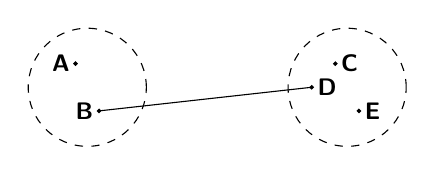
\begin{tikzpicture}[sloped,scale=0.3,every node/.style={scale=0.6}] %first scales the image, second scales nodes/fonts
   %\draw[help lines] (-8,0) grid +(16,4); %showing grid is helpful to determine coordinates
   \draw [fill] (-6,3) circle (2pt) coordinate(a) node[anchor=east] {A};
   \draw [fill] (-5,1) circle (2pt) coordinate(b) node[anchor=east] {B};
   \draw [fill] (5,3) circle (2pt) coordinate(c) node[anchor=west] {C};
   \draw [fill] (4,2) circle (2pt) coordinate(d) node[anchor=west] {D};
   \draw [fill] (6,1) circle (2pt) coordinate(e) node[anchor=west] {E};
    \draw  (b) -- (d);
    \draw [dashed] (-5.5,2) circle [radius=2.5];
    \draw [dashed] (5.5,2) circle [radius=2.5];
\end{tikzpicture}              
% \vfill
\pause
    \item \alert{\bf Complete linkage}:\\
     { \small
		maximum distance or farthest neighbor (2 farthest border points)
    }
    % \vfill
    \pause

      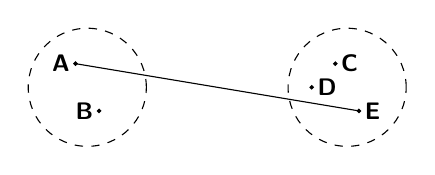
\begin{tikzpicture}[sloped,scale=0.3,every node/.style={scale=0.6}]
   \draw [fill] (-6,3) circle (2pt) coordinate(a) node[anchor=east] {A};
   \draw [fill] (-5,1) circle (2pt) coordinate(b) node[anchor=east] {B};
   \draw [fill] (5,3) circle (2pt) coordinate(c) node[anchor=west] {C};
   \draw [fill] (4,2) circle (2pt) coordinate(d) node[anchor=west] {D};
   \draw [fill] (6,1) circle (2pt) coordinate(e) node[anchor=west] {E};
    \draw  (a) -- (e);
    \draw [dashed] (-5.5,2) circle [radius=2.5];
    \draw [dashed] (5.5,2) circle [radius=2.5];
  \end{tikzpicture}
  \pause
    \item \alert{\bf Average linkage (unweighted pair-group method)}:\\
     { \small
average distance (all to all)
	}
 
     \pause

        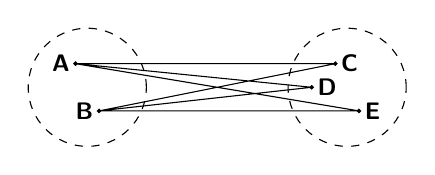
\begin{tikzpicture}[sloped,scale=0.3,every node/.style={scale=0.6}]
   \draw [fill] (-6,3) circle (2pt) coordinate(a) node[anchor=east] {A};
   \draw [fill] (-5,1) circle (2pt) coordinate(b) node[anchor=east] {B};
   \draw [fill] (5,3) circle (2pt) coordinate(c) node[anchor=west] {C};
   \draw [fill] (4,2) circle (2pt) coordinate(d) node[anchor=west] {D};
   \draw [fill] (6,1) circle (2pt) coordinate(e) node[anchor=west] {E};
    \draw  (a)--(c) (a)--(d) (a)--(e) (b)--(c) (b)--(d) (b)--(e);
    \draw [dashed] (-5.5,2) circle [radius=2.5];
    \draw [dashed] (5.5,2) circle [radius=2.5];
\end{tikzpicture}
   \end{itemize}
    
\end{frame}
 
%%% SLIDE LAYOUT EXAMPLE
\begin{frame}[shrink=25]
\frametitle{Agglomerative clustering algorithm}
\begin{minipage}[]{.45\textwidth}
\centering
 \begin{tikzpicture}[node distance = 1cm, auto]
   % Place nodes
   \visible<4->{\node [block] (init) {create \textit{N} singleton clusters};}
   \visible<2->{\node [cloud, left=of init] (strt) {start};}
   \visible<6->{\node [block, below=of init] (merge) {merge two most similar clusters};}
   \visible<8->{\node [block, below=of assign] (update) {update between-cluster distances};}
   \visible<10->{\node [decision, below=of update] (decide) {only one cluster left?};}
   \visible<12->{\node [cloud, right=of decide] (stop) {stop};}
   % Draw edges
   \visible<3->{\path [line] (strt) -- (init);}
   \visible<5->{\path [line] (init) -- (merge);}
   \visible<7->{\path [line] (merge) -- (update);}
   \visible<9->{\path [line] (update) -- (decide);}
   \visible<12->{\path [line] (decide) -- node {yes} (stop);}
   \visible<11->{\path [line] (decide)  --++  (-3,0) node [near start] {no} |- (merge);}
 \end{tikzpicture}
\end{minipage}\hfill\pause
\begin{minipage}[]{.5\linewidth}
  \centering

  Example:
  \pause
  
  \visible<+->{\includegraphics[width=.72\textwidth,trim={5.1in 0 0 0}, clip]{dendrogram}}
  \pause
  
  \visible<+->{\includegraphics[width=.72\textwidth,trim={0 0 5.2in 0}, clip]{dendrogram}}

  {\tiny Source: James et Al., Introduction to Statistical Learning}
\end{minipage}
\end{frame}
 
\begin{frame}
\frametitle{Choosing the clusters}
We decide a \alert{Cut}\\
  \includegraphics[width=\textwidth]{from_dendrogram_to_clusters}
	\begin{tiny}Source: James et Al., Introduction to Statistical Learning\end{tiny}\\
%No (Sec. 10.3.2 of Introduction to Statistical Learning)
\end{frame}

% \begin{frame}
% \frametitle{Hierarchical Clustering: Dendrogram}
%   \includegraphics[width=\textwidth]{dendrogram}
% %	\tiny{Source: James et Al., Introduction to Statistical Learning}
% \vspace{-0.7cm}
% \begin{small}
% \begin{columns}[T]
% \begin{column}{0.50\columnwidth}
%  \begin{itemize}
% 	\item Distance in the y axis
% 	\item Distance between 5 and 7? And between \{5,7,8,2\} and \{ 9 \}?
%  \end{itemize}
% \end{column}
% \begin{column}{0.50\columnwidth}
%  \begin{itemize}
% 	\item Are 2 and 9 ``close''? Distance between 2 and 9?
% 			%cannot tell%
% 			Distance between \{5,7,8\} and \{9\}?
% 			%cannot tell%
%   \end{itemize}
% \end{column}
% \end{columns}
% \end{small}
% \end{frame}
 
\begin{frame}%[shrink=1]
\frametitle{Practical Considerations}
Advantages
 \begin{itemize}
 \item No apriori number of clusters required
 \item Simple algorithms
 \item Self-organized structural view of data
   \end{itemize}
   Disadvantages
    \begin{itemize}
    \item Dendrogram often difficult to visualize
    \item Sometimes the inherent clusters in our data are not hierarchical by nature (K-means performs better in these cases)
   \end{itemize}
\end{frame}



%\begin{frame}%[shrink=1]
%\frametitle{Practical Considerations}
% \begin{itemize}
% \setlength{\itemindent}{-1em}
%   \item Missing data.
%   \begin{itemize}
%   \setlength{\itemindent}{-1em}
%   \item Clustering methods demand complete data.
%   \end{itemize}
%   \item Outliers.
%   \begin{itemize}
%    \setlength{\itemindent}{-1em}
%   \item Centroid-based clustering such as $K$-means is very sensitive to outliers.
%   \end{itemize}
%   \end{itemize}
%  \begin{columns}[T] % contents are top vertically aligned
%   \begin{column}{0.48\textwidth}%[T]{0.5\textwidth}
%   %\setlength{\itemindent}{5em}
%   \begin{itemize}
%   \item Cluster shapes
%   \begin{itemize}
%   \item Centroid-based clustering is not suitable for non-convex (non-ellipsoidal) cluster shapes.\\
%   \end{itemize}
%   \end{itemize}
%   \end{column}
%   \begin{column}{0.48\textwidth}%[T]{0.5\textwidth} % alternative top-align that's better for graphics
%   \includegraphics[width=3.5cm]{clustershape}
%   \newline
%   \tiny{Source: Wikipedia}
%   \end{column}
%  \end{columns}
%\end{frame}


\begin{frame}
  \frametitle{HAC example: Bicycle ownership trends}
  Pattern discovery from survey data in 150 countries spanning 30 years \footnote{Oke et al., 2015 \url{https://www.sciencedirect.com/science/article/abs/pii/S2214140515006787}}
  % \begin{itemize}
  % \item
  % \item Pattern discovery in bicycle ownership
  % \end{itemize}

  \begin{columns}
    \begin{column}{.7\textwidth}
    \includegraphics[width=.475\linewidth]{fig-weightedfit-G1}
    \includegraphics[width=.475\linewidth]{fig-weightedfit-G2}
    
    \includegraphics[width=.475\linewidth]{fig-weightedfit-G3}  
    \includegraphics[width=.475\linewidth]{fig-weightedfit-G4}      
    \end{column}
    \begin{column}{.3\textwidth}
      \begin{block}{Key findings}\small
        \begin{itemize}
        \item To cluster time-series data of varying lengths,
          the dynamic time warping (DTW) algorithm can be used to compute the dissimilarity matrix
        \end{itemize}
      \end{block}
     \includegraphics[width=1\textwidth,height=.6\textwidth]{gbo_map}
      \end{column}
  \end{columns}  
 
\end{frame}





\section{DBSCAN}
\begin{frame}
  \frametitle{Density-based clustering}
  Density-based clustering approaches are based on these hypotheses:
  \begin{itemize}
  \item Clusters are dense spatial regions
  \item Clusters are separated by low-density regions
  \item The density of points in a cluster are greater than a given minimum
  \end{itemize}
  \pause
  Examples of density-based clustering algorithms:\pause
  \begin{itemize}
  \item DBSCAN
  \item OPTICS
  \end{itemize}
\end{frame}

\begin{frame}
  \frametitle{Density-based spatial clustering of applications with noise}\pause
  \pause
  \begin{itemize}\pause
  \item Introduced in 1996 by Ester, Kriegel, Sander \& Xu\footnote{\url{https://citeseerx.ist.psu.edu/viewdoc/summary?doi=10.1.1.121.9220}}
  \item Finds dense regions; recursively expands them to converge at clusters\pause
  \item Parameters:\pause
    \begin{itemize}
    \item $\varepsilon$: radius of neighborhood\pause
    \item $\text{minPoints}$: minimum number of observations within a neighborhood\pause
    \end{itemize}
  \end{itemize}
  \pause
  \visible<+->{
    \begin{figure}
      \centering
     \includegraphics[width=.9\textwidth,trim={0 17in 0 0}, clip]{dbscanfig}

     {\tiny Source: \url{https://www.nature.com/articles/srep34406}}
     \caption{Example of clusters generated by DBSCAN on a dataset}
   \end{figure}
 }
\end{frame}

\begin{frame}
  \frametitle{DBSCAN: key definitions}
  \pause

  \begin{minipage}[t]{.6\linewidth}
  \begin{itemize}
  \item Epsilon neighborhood, $N_{\varepsilon}$: set of all observations within distance $\varepsilon$
  \item Core point: has at least \texttt{minPoint} observations within its  $N_{\varepsilon}$
  \item DDR: An observation $j$ is \textbf{directly density reachable} from a core point $i$ if $j\in  N_{\varepsilon}$
  \item DR: Two observations are \textbf{density reachable} if there exists a chain of DDR observations linking them
  \item Boundary/border points: these are DDR but not core points
  \item Noise/outlier points: do not belong to any observations  $N_{\varepsilon}$
  \end{itemize}
\end{minipage}\hfill
\begin{minipage}[t]{.35\linewidth}
  \visible<+->{
    \begin{figure}
      \centering
      \includegraphics[width=.8\textwidth]{dbscan-min4}

      {\tiny Source: Giacoumidis et al. (2019) \url{https://www.mdpi.com/2076-3417/9/20/4398/htm}}
      \caption{DBSCAN example with minpoints = 4}
    \end{figure}
  }
\end{minipage}

\end{frame}
\begin{frame}[shrink=20]
  \frametitle{DBSCAN serial algorithm}\small
  \pause
%\begin{algorithm}[H]
 %  \caption{DBSCAN serial algorithm}\label{dbserial}
  \begin{algorithmic}[1]
    \Procedure{DBSCAN}{$X,\varepsilon, \text{minPoints}$} 
      \For{each unvisited point $x\in X$}
         \State mark $x$ as visited
         \State $N \leftarrow$ \textsc{FindNeighbors}$(x, \varepsilon)$
         \If{$|N| < \text{minPoints}$}
             \State mark $x$ as noise
         \Else
             \State $C \leftarrow \{x\}$
         \EndIf
         \For{each point $x' \in N$}
             \State $N \leftarrow N\setminus x'$
             \If{$x'$ is not visited}
                  \State mark $x'$ as visited
                  \State $N' \leftarrow$ \textsc{FindNeighbors}$(x', \varepsilon)$
                  \If{$|N'| \ge \text{minPoints}$}
                       \State $N\leftarrow N \cup N'$
                  \EndIf 
             \EndIf 
             \If{$x'$ is not yet a member of any cluster}
                  \State $C\leftarrow C\cup\{x'\}$
             \EndIf
         \EndFor
      \EndFor
    \EndProcedure
   \end{algorithmic}
%\end{algorithm}
\end{frame}

\begin{frame}
\frametitle{DBSCAN example: stop detection}\pause
\begin{itemize}[<+->]
\item \alert{Stop detection} using smartphone data. \vskip5pt
\item \alert{Challenges:} GPS data is noisy. Data gaps (e.g. no GPS inside buildings). \vskip5pt
%\item \alert{Example:} \emph{Future Mobility Sensing (FMS)}
\end{itemize}

\begin{figure}
    \centering
        \includegraphics[width=0.4\textwidth]{FMS-raw}  %image width relative to textwidth
    \includegraphics[width=0.4\textwidth]{FMS-dbscan3}  
  \end{figure}
\end{frame}

% \begin{frame}
% \frametitle{Clustering Applications: Transportation}
%  \begin{figure}
%   \centering
%   \includegraphics[width=0.7\textwidth]{FMS-dbscan3}  
%    %\caption{Optional figure caption}
%    %\label{fig:mitlogo}
%  \end{figure}
% \end{frame}



\begin{frame}
  \frametitle{DBSCAN considerations}
  \pause
  \begin{itemize}
  \item Performs well on geographical data

  \item Requires careful selection of two parameters (can be computationally intensive)
    
  \item Several improvements and updates to the original DBSCAN algorithm have been made (e.g. OPTICS: ``Ordering points to identify the clustering structure'')

  \end{itemize}
\end{frame}

\section{Silhouette}

\begin{frame}
  \frametitle{Fitness of clustering solution}
 %\setlength{\itemindent}{-1em}
Good clustering should:
   \begin{itemize}
   \item Minimize \alert{within-cluster} (inter-cluster) variability~($\textbf{W}$)
	%\[ \min \sum_{k=1}^K \sum_{\mathbf{z}\in C_k} d(\mathbf{z},\bar{\mathbf{z}}_k)^2 \]
   \item Maximize the \href{https://www.sciencedirect.com/science/article/pii/0377042787901257}{silhouette (Rousseeuw, 1987)}

   \item Several other goodness-of-fit measures can be used:
     \begin{itemize}
     \item \href{https://www.jstor.org/stable/pdf/2531893.pdf}{Krzanowski-Lai (KL) index}
     \item \href{https://statweb.stanford.edu/~gwalther/gap}{Gap statistic (Tibshirani et al., 2001)}
     \end{itemize}

   \item We consider the silhouette metric in detail
  \end{itemize}
\end{frame}








\begin{frame}
  \frametitle{Silhouette}
 \begin{itemize}[<+->]
   \item Silhouette of observation $\textbf{x}_j$, $s(\textbf{x}_j)$:
     \begin{equation}
   s(\textbf{x}_j)=\frac{b(\textbf{x}_j)-a(\textbf{x}_j)}{\max\{a(\textbf{x}_j), b(\textbf{x}_j)\}}
 \end{equation}

   \item $a(\textbf{x}_j)$= average distance between $\textbf{x}_j$ and \emph{all} other elements of its cluster (intra-cluster distance)
   \item $b(\textbf{x}_j)$= average distance between $\textbf{x}_j$ and \emph{all} elements of the second nearest cluster.

     
   \item Measures how well an observation fits a cluster
     \begin{equation}
   -1<s(\textbf{x}_j)<1
 \end{equation}

   \item We want $a(\textbf{x}_j)$ to be small and $b(\textbf{x}_j)$ to be large:
     \begin{equation}
   a(\textbf{x}_j)\ll b(\textbf{x}_j) \pause \implies \pause s(\textbf{x}_j) \rightarrow 1
 \end{equation}

  \end{itemize}
  
\end{frame}

\begin{frame}{Silhouette: visualization}
\begin{columns}[T]
\begin{column}{0.70\textwidth}
    \includegraphics[width=.9\textwidth]{silhouette}\\
\end{column}
\begin{column}{0.3\textwidth}
\tiny{source:Scikit-learn: \url{scikit-learn.org/stable/auto/examples/cluster/plot_kmeans_silhouette_analysis.html} } 
\end{column}
\end{columns}
\end{frame}




\section{Summary}

\begin{frame}[fragile]
  \frametitle{Outlook}
  \pause

  \begin{itemize}[<+->]
  \item Assigned reading: ISLR 10.3, 10.4
    \item Further recommended reading: ESL 14.3
  \end{itemize}
\end{frame}

%\appendix\addtocounter{part}{-1}

 
\end{document}

%%% Local Variables:
%%% mode: latex
%%% TeX-master: t
%%% End:
